%!TeX program=lualatex

\documentclass{homework}
% \usepackage{lua-visual-debug}
% \usepackage[a4paper, total={6in, 8in}]{geometry}
\usepackage{graphicx}
\usepackage{float}
\usepackage{hyperref}
\usepackage{enumitem}
\usepackage{ulem}
\usepackage{amsmath}

\title{Wireshark \#2}
\subject{CS341 Introduction to Computer Networks}
\studentid{20170058}
\name{Keonwoo Kim}
\date{\today}

\setstretch{1.0}

\begin{document}
\maketitle

\solution{(UDP) [Refer \texttt{/tmp/wireshark\_any\_20201029172154\_pP9xGd.pcapng} below.]

\begin{enumerate}[label={(\arabic*)}]
 \item Select one UDP packet from your trace. From this packet, determine how many fields there are in the UDP header. (You shouldn’t look in the textbook! Answer these questions directly from what you observe in the packet trace.) Name these fields.
 
 \textit{[Answer]} There are 4 fields in the UDP header: \uline{\texttt{Source Port}, \texttt{Destin-} \texttt{ation Port}, \texttt{Length}, and \texttt{Checksum}.}
 
 \item By consulting the displayed information in Wireshark’s packet content field for this packet, determine the length (in bytes) of each of the UDP header fields.
 
 \textit{[Answer]} Each field has a length of \uline{2 bytes}.
 
 \item What is the maximum number of bytes that can be included in a UDP payload? (Hint: the answer to this question can be determined by your answer to 2. above)
 
 \textit{[Answer]} Since the \texttt{Length} field is of length 2 bytes, which is 16 bits, the maximum length of a packet is $2^{16}-1 = 65535$ [bytes]. Since the UDP header takes 8 bytes (from 1. and 22.), the maximum number of bytes that can be included in a UDP packet is $65535 - 8 =$\,\uline{$65527$ [bytes]}.
 
 \item Examine a pair of UDP packets in which your host sends the first UDP packet and the second UDP packet is a reply to this first UDP packet. (Hint: for a second packet to be sent in response to a first packet, the sender of the first packet should be the destination of the second packet). Describe the relationship between the port numbers in the two packets.
 
 \textit{[Answer]} The source port of the reply packet is the same with the destination port of the first packet, and the destination port of the reply packet is the same with the source port of the first packet.
\end{enumerate}
}


\newpage 

\solution{(TCP) [Refer \texttt{/tmp/wireshark\_wlp1s0\_20201029190844\_2WuBOQ.pcapng} below.]

\begin{enumerate}[label={(\arabic*)}]
 \item What is the IP address and TCP port number used by your client computer (source) to transfer the file to gaia.cs.umass.edu?
 
 \textit{[Answer]} The IP address is \texttt{192.168.0.107}, and the TCP port number is \texttt{60286}.

 
 \item What is the sequence number of the SYNACK segment sent by gaia.cs.umass.edu to the client computer in reply to the SYN? What is the value of the Acknowledgement field in the SYNACK segment? How did gaia.cs.umass.edu determine that value? What is it in the segment that identifies the segment as a SYNACK segment?
 
 \textit{[Answer]} The sequence number of the SYNACK segment is \texttt{2050667101} (\texttt{0x7a3ab25d},) and the value of the acknowledgement field in the SYNACK segment is \texttt{39762633} (\texttt{0x025ebac9}.) This value is determined by adding 1 to the sequence number of the SYN segment sent by the client.
 
  The SYNACK segment is realized by the flags set, where the flags \texttt{0x12} mean that the acknowledgement flag and Syn flag are set as shown below.

 \begin{center}
  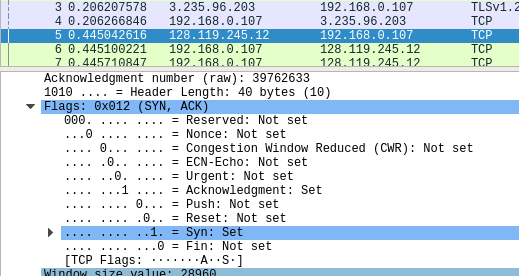
\includegraphics[width=0.8\textwidth]{Screenshot from 2020-10-29 19.32.53.png}
 \end{center}
 
 \item What is the sequence number of the TCP segment containing the HTTP POST command? Note that in order to find the POST command, you’ll need to dig into the packet content field at the bottom of the Wireshark window, looking for a segment with a “POST” within its DATA field.
 
 \textit{[Answer]} The sequence number of the TCP segment containing the HTTP POST command is \texttt{39762633} (\texttt{0x025ebac9}.)
 
 \item What is the throughput (bytes transferred per unit time) for the TCP connection? Explain how you calculated this value.
 
 \textit{[Answer]} The last ACK number of the TCP connection is \texttt{39913225}. Therefore, since the TCP segment containing the HTTP POST command is sent, the client have sent $39913225 - 39762633 = 150592$ [bytes]. Note that the time difference between two segments is $3.006507397 - 0.241993047 = 2.76451435$ [seconds]. Therefore, the average throughput of the TCP connection is
 \begin{align*}
  150592\text{\,[bytes]}/2.76451435\text{\,[seconds]} &= 54473.2205857\text{\,[bytes/second]} \\&= \uline{435.785764686 \text{\,[kbps].}}
 \end{align*}
 

\end{enumerate}
}


\end{document}